\documentclass[tikz,border=6pt,12pt]{standalone}
\usetikzlibrary{arrows.meta, positioning, calc, backgrounds}
\definecolor{navy}{HTML}{003057}
\definecolor{gold}{HTML}{B3A369}
\definecolor{shared}{HTML}{5F7794}
\definecolor{grey}{HTML}{A0A0A0}
\begin{document}
\sffamily
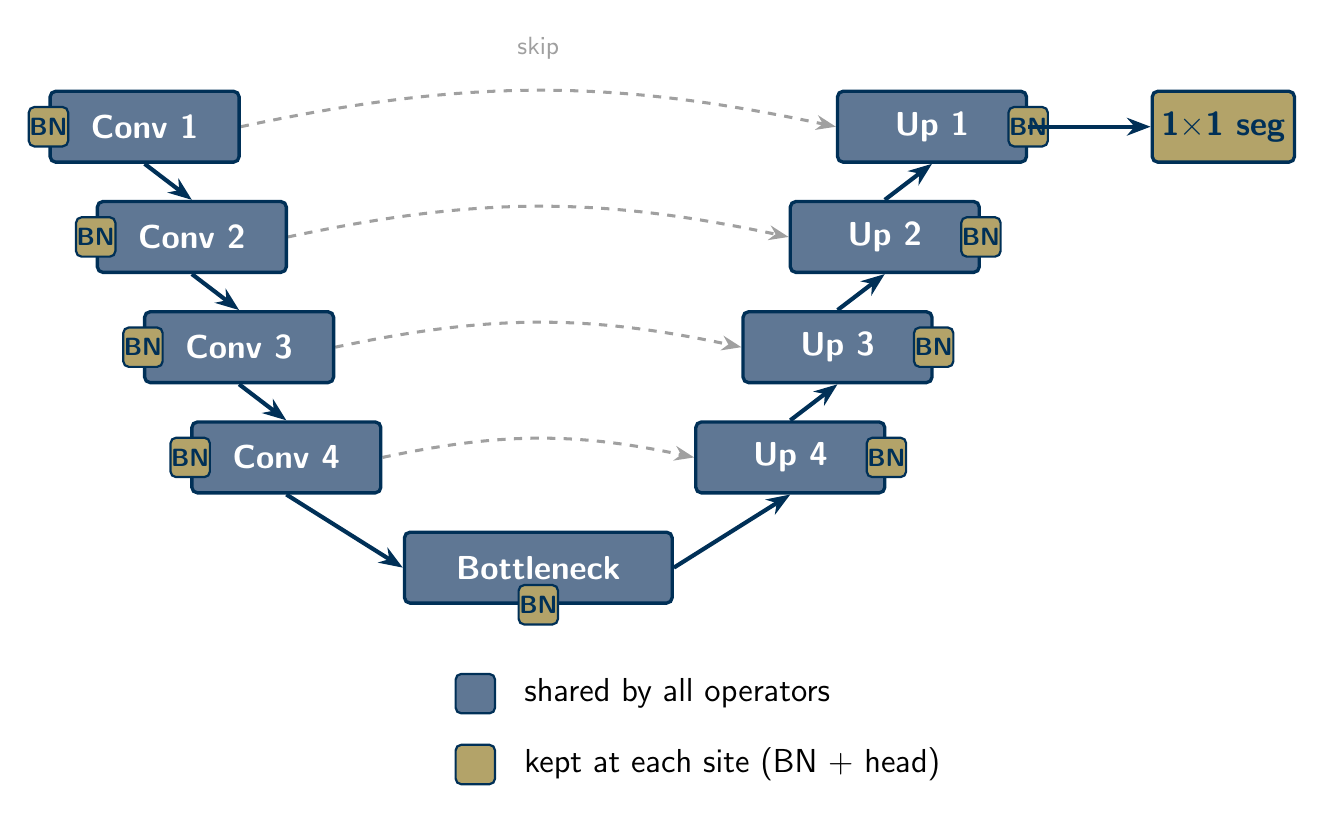
\begin{tikzpicture}[
  every node/.style={font=\sffamily\large},
  block/.style={rectangle, fill=shared, draw=navy, line width=1.2pt,
                 rounded corners=2pt, minimum width=2.4cm, minimum height=0.9cm,
                 text=white, font=\sffamily\large\bfseries, align=center},
  bn/.style={rectangle, fill=gold, draw=navy, line width=0.8pt, rounded corners=2pt,
              minimum width=0.5cm, minimum height=0.5cm, inner sep=0pt,
              text=navy, font=\sffamily\small\bfseries},
  head/.style={rectangle, fill=gold, draw=navy, line width=1.2pt,
                rounded corners=2pt, minimum width=1.7cm, minimum height=0.9cm,
                text=navy, font=\sffamily\large\bfseries},
  arr/.style={-{Stealth[length=3mm]}, line width=1.5pt, draw=navy},
  skip/.style={-{Stealth[length=2.5mm]}, line width=1.1pt, draw=grey, dashed},
]
% ---- encoder (down the left) ----
\node[block] (c1) at (0,0)   {Conv 1};
\node[block] (c2) at (0.6,-1.4) {Conv 2};
\node[block] (c3) at (1.2,-2.8) {Conv 3};
\node[block] (c4) at (1.8,-4.2) {Conv 4};
% ---- bottleneck ----
\node[block, minimum width=3.4cm] (bot) at (5,-5.6) {Bottleneck};
% ---- decoder (up the right) ----
\node[block] (u4) at (8.2,-4.2) {Up 4};
\node[block] (u3) at (8.8,-2.8) {Up 3};
\node[block] (u2) at (9.4,-1.4) {Up 2};
\node[block] (u1) at (10,0)  {Up 1};
% ---- head (local) ----
\node[head] (hd) at (13.7,0) {1$\times$1 seg};
% ---- BN badges (local): west of encoder, east of decoder, on bottleneck ----
\foreach \n in {c1,c2,c3,c4}{ \node[bn] at (\n.west) {BN}; }
\foreach \n in {u1,u2,u3,u4}{ \node[bn] at (\n.east) {BN}; }
\node[bn] at (bot.south) {BN};
% ---- main path ----
\draw[arr] (c1.south) -- (c2.north);
\draw[arr] (c2.south) -- (c3.north);
\draw[arr] (c3.south) -- (c4.north);
\draw[arr] (c4.south) -- (bot.west);
\draw[arr] (bot.east) -- (u4.south);
\draw[arr] (u4.north) -- (u3.south);
\draw[arr] (u3.north) -- (u2.south);
\draw[arr] (u2.north) -- (u1.south);
\draw[arr] (u1.east) -- (hd.west);
% ---- skip connections (grey, under the badges) ----
\begin{scope}[on background layer]
  \draw[skip] (c1.east) to[bend left=12] (u1.west);
  \draw[skip] (c2.east) to[bend left=12] (u2.west);
  \draw[skip] (c3.east) to[bend left=12] (u3.west);
  \draw[skip] (c4.east) to[bend left=12] (u4.west);
\end{scope}
\node[font=\sffamily\small, text=grey] at (5,1.0) {skip};
% ---- legend (stacked, two rows) ----
\node[rectangle, fill=shared, draw=navy, line width=0.8pt, rounded corners=2pt, minimum height=0.5cm, minimum width=0.5cm, inner sep=0pt] at (4.2,-7.2) {};
\node[anchor=west, font=\sffamily\large] at (4.7,-7.2) {shared by all operators};
\node[bn, minimum height=0.5cm, minimum width=0.5cm] at (4.2,-8.1) {};
\node[anchor=west, font=\sffamily\large] at (4.7,-8.1) {kept at each site (BN + head)};
\end{tikzpicture}
\end{document}
